\subsection{Brake Controller}

A brake controller is a crucial component in autonomous and assisted driving systems, enabling vehicles to respond intelligently to detected obstacles or hazards.
In this project, a simple yet effective braking mechanism was implemented using a linear controller that calculates a safe stopping distance based on the vehicle's current speed.
The controller assumes a linear relationship between speed and stopping distance, a reasonable approximation under controlled conditions and for the rather lightweight go-kart.
The controller's objective is to ensure that if the vehicle is approaching an obstacle inside an area of interest and potentially getting into contact with it, it activates the brake early enough to stop within a safe distance.
Here, the area of interest is a specified area in front of the go-kart encasing the space where an approaching stationary obstacle could become a hazard to the driver and vehicle.
As the distance which is required to stop the vehicle before getting into contact with the obstacle is proportional to the vehicle's speed, the length of the area of interest is coupled to it.
\par
The brake controller's logic is based on the following variables:
\begin{itemize}
    \item Stopping distance $d_{\text{stop}}(v_{\text{current}})$: Estimates how much distance the vehicle requires to come to a complete stop at the current speed, according to the vehicle specifications.
    \item Output signal $brake\_signal(d_{\text{stop}},d_{\text{target}})$: Generates a binary brake signal (0 or 1) based on whether the stopping distance exceeds the target distance. As the current brake controller simply considers if the brake should be applied or not.
\end{itemize}
The stopping distance is computed relative to a reference speed and stopping distance (default: 40~kph $\rightarrow$ 6~meters), allowing for linear scaling:
\[
d_{\text{stop}}(v_{\text{current}}) = \frac{v_{\text{current}}}{v_{\text{ref}}} \cdot d_{\text{ref}}
\]
If the required stopping distance is greater than or equal to the available distance (measured distance to a detected obstacle), the system triggers full braking:
\[
brake\_signal(d_{\text{stop}},d_{\text{target}}) =
\begin{cases}
1 & \text{if } d_{\text{target}} \leq d_{\text{stop}} \\
0 & \text{otherwise}
\end{cases}
\]

\begin{figure}[!htbp]
    \centering
    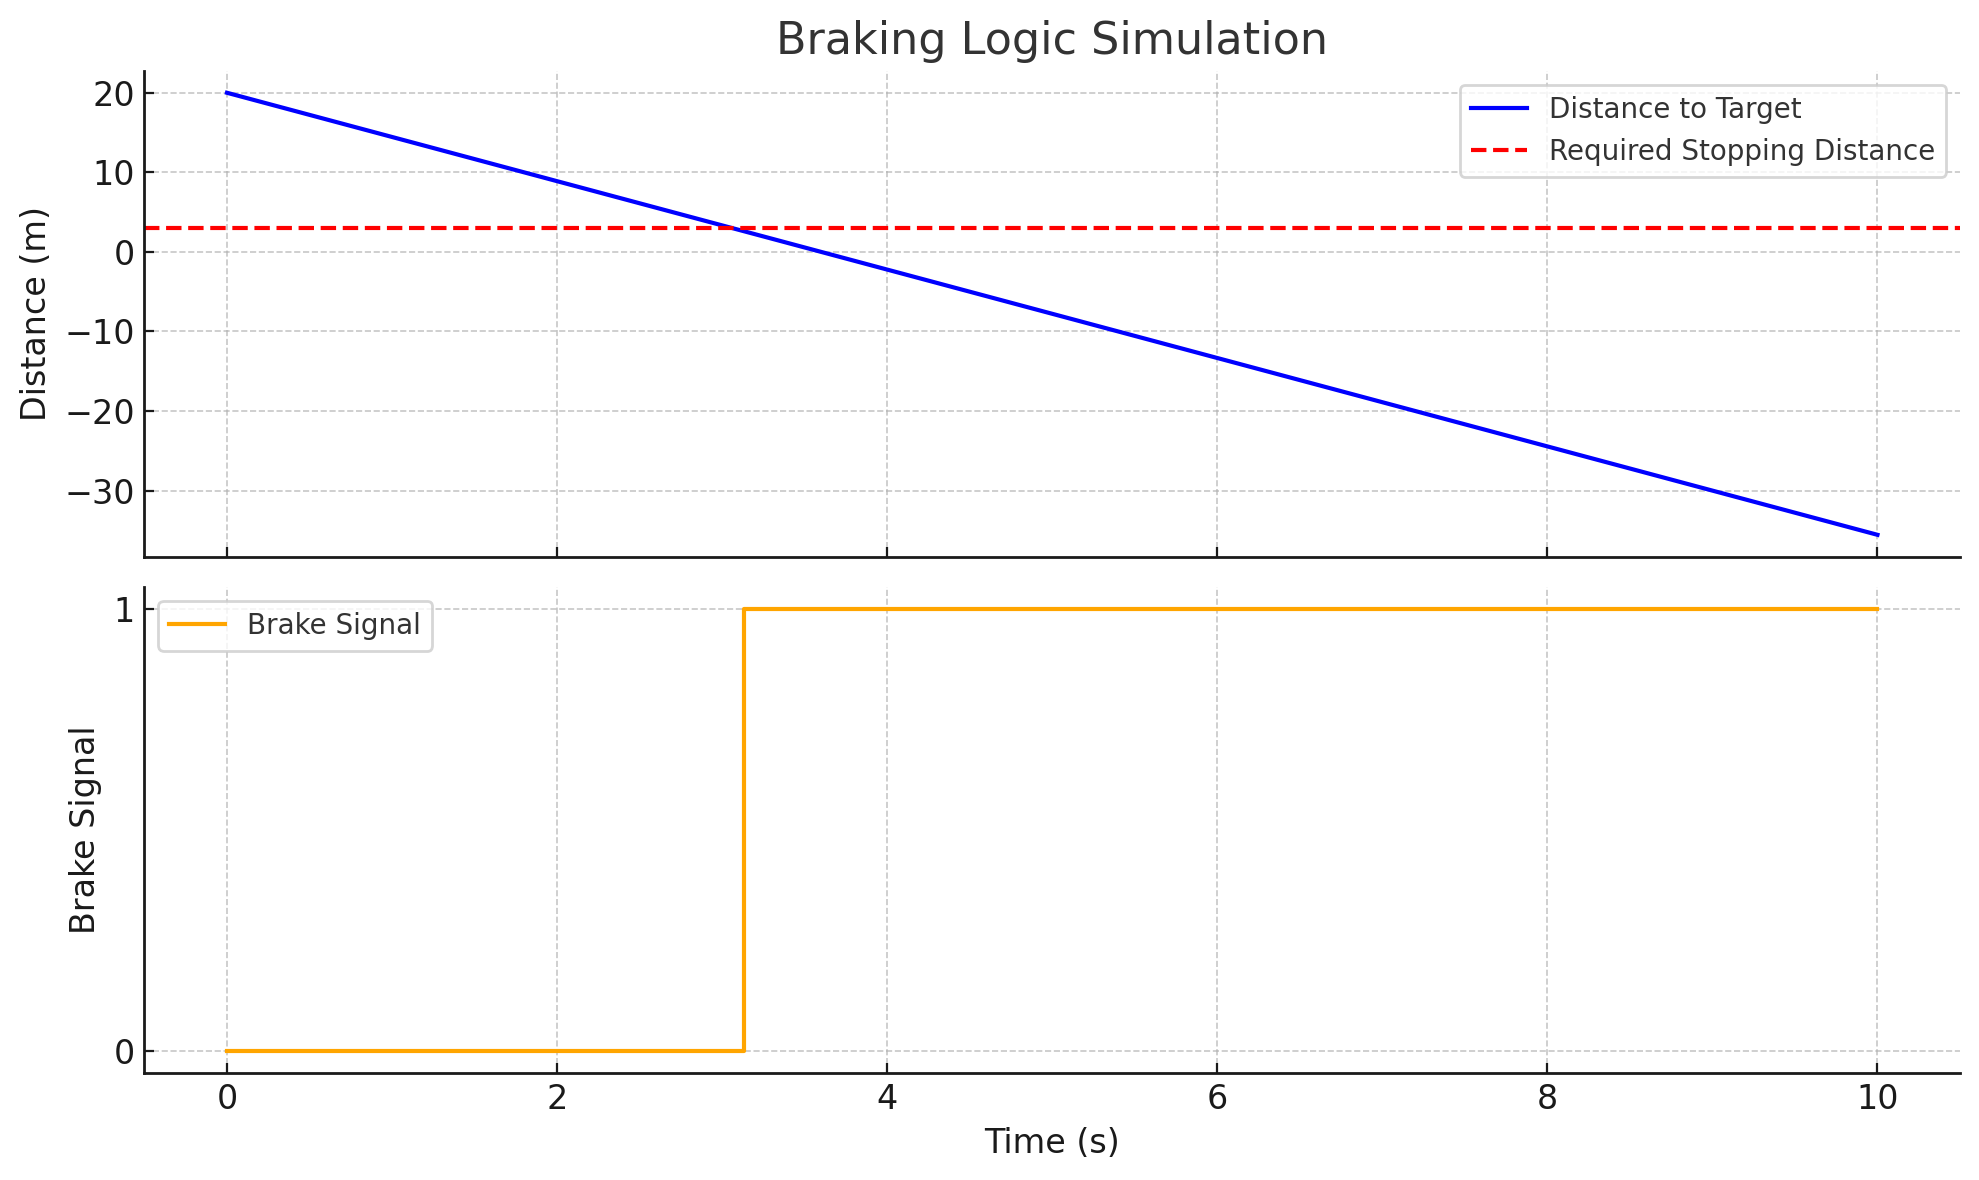
\includegraphics[width=0.8\linewidth]{images/brakeSignal.png}
    \caption{Braking decision based on stopping distance estimation.}
    \label{fig:braking_logic}
\end{figure}
This straightforward logic allows the controller to make quick decisions in real time, helping the vehicle to react safely to moving and stationary objects, detected by the radar.
Although the system is designed to be cautious because it only switches between braking and not braking, it could be improved later by adding smoother braking or more advanced features like adaptive cruise control.
The controller plays a key role in the interaction between detection (from the radar sensor's output data and the processing pipeline) and actuation (braking), forming the basis for a closed-loop safety mechanism.